% В этом шаблоне используется класс spbau-diploma. Его можно найти и, если требуется, 
% поправить в файле spbau-diploma.cls
\documentclass{spbau-diploma}
\begin{document}
\filltitle{ru}{
    chair              = {Кафедра математических и информационных технологий},
    title              = {Анализ смесей близкородственных
бактериальных штаммов в метагеномных~сериях},
    type               = {master},
    position           = {студента},
    group              = 605,
    author             = {Аксешина Маргарита Дмитриевна},
    supervisorPosition = {},
    supervisor         = {Нурк С.\,Ю.},
    reviewerPosition   = {к.\,т.\,н},
    reviewer           = {Казаков С.\,В.},
    chairHeadPosition  = {д.\,ф.-м.\,н., профессор},
    chairHead          = {Омельченко А.\,В.},
}


\maketitle


\tableofcontents


% ВВЕДЕНИЕ
\section*{Введение}

\subsection{Введение в область} 

Изучение мира микробов (микроорганизмов) является критически важным для понимания многих аспектов жизни на Земле. Циклы химических реакций, преобразующие ключевые элементы жизни --- углерод, азот, кислород и серу --- в биологически доступные формы, в значительной степени зависят от микробов \cite{metabook}. Все растения и животные тесно связаны с микробными сообществами, продуцирующими необходимые для жизни их хозяев питательные вещества, металлы и витамины \cite{microbes_animals}. Благодаря ферментации и другим естественным процессам микробы создают или добавляют ценность многим продуктам питания человека. Микробы также устраняют токсины в окружающей среде --- и те, которые производятся естественным путем, и те, которые являются побочными продуктами человеческой деятельности, такие как нефтяные и химические разливы \cite{oil}. 

\textit{Геном} --- это совокупность наследственного материала организма. Информация генома обычно закодирована в молекулах дезоксирибонуклеиновой кислоты (ДНК). Молекула ДНК состоит из последовательности нуклеотидов четырёх типов: аденин (А), гуанин (G), цитозин (С) и тимин (Т).

\textit{Ген} --- участок ДНК, определяющий возможность развития отдельного элементарного признака. В случае бактерий ген можно представить как непрерывную последовательность нуклеотидов, встречающихся в геноме.

\textit{Секвенирование} --- это общее название методов, которые позволяют установить последовательность нуклеотидов в молекуле ДНК. 

\textit{Метагеномика} изучает микробные сообщества посредством секвенирования ДНК, полученной непосредственно из образцов среды, минуя этапы выделения и культивирования микроорганизмов. Метагеномика позволяет исследовать как видовое, так и функциональное разнообразие микробных сообществ \cite{HMP1, HMP2}. 
Кроме того, метагеномика предоставляет доступ к геномам микроорганизмов, которые на данный момент не поддаются культивации.
% * <novmargo@gmail.com> 03:11:33 13 Jun 2018 UTC+0300:
% ОЦЕНКА НА ТО, СКОЛЬКО НЕ ПОДДАЁТСЯ КУЛЬТИВАЦИИ СО ССЫЛКОЙ.

Биологические объекты метагеномики --- это бактерии, археи, вирусы, эукариоты (грибы, примеси ДНК хозяина). Но в данной работе мы сосредоточимся на бактериальных геномах и под словом \textit{микроорганизмы} также будем понимать бактерии.

Активному развитию метагеномики в последнее десятилетие в значительной степени способствовало появление методов \textit{секвенирования нового поколения}. Их результатом является набор коротких (обычно 100-250 нуклеотидов) геномных фрагментов --~\textit{ридов}. 

Важные функциональные элементы генома (гены, регуляторные участки, повторы и т.д.) обычно не умещаются в один рид. 
С целью проведения дальнейшего анализа многие современные исследования предварительно объединяют риды в более длинные последовательности исходных геномов -- \textit{контиги}. 
Для этого используются специализированные программные инструменты -- метагеномные сборщики (\cite{IDBA-UD, MEGAHIT, MetaVelvet, RayMeta, MetaSpades}). Кроме контигов эти программы могут выдавать \textit{граф сборки}, отражающий связи между контигами (подробнее о графе сборки будет сказано ниже).

За этапом сборки обычно следует этап \textit{биннинга}, -- то есть разделение полученных контигов на группы, в идеале соответствующие отдельным микроорганизмам. Инструменты для биннинга \cite{CONCOCT, GroopM, MyCC, MetaBAT} основываются на анализе состава нуклеотидных последовательностей (например, тетрануклеотидном <<спектре>>), а также глубины их покрытия в образце. 
Важным преимуществом подхода, основанного на сборке и биннинге, над методами метагеномного анализа видового состава образцов, является возможность функциональной аннотации генома конкретной популяции того или иного вида, присутствующего в данном образце. % (или каждом из образцов серии, при наличии таковых).

Отметим также, что многие современные исследования включают анализ множества образцов, формирующих \textit{метагеномные серии} (пробы одного и того же сообщества, полученные в разные момент времени \cite{time_series} или в близких локациях ~\cite{spacial_series_1, spacial_series_2}). Хотя такие данные исходно предназначаются для того, чтобы отследить динамику изменения сообщества, наличие иформации о совместном покрытии контигов в каждом из образцов помогает значительно улучшить качество биннинга \cite{CONCOCT}.


\subsection{Штаммы близкородственных видов}

Различные геномные варианты одного вида бактерии называют \textit{штаммами}. Вариации между геномами штаммов обычно состоят из однонуклеотидных мутаций, а также приобретений/потерь геномных элементов, включая гены, опероны или плазмиды \cite{StrainPhlAn}. Различные штаммы одного вида микроорганизма могут сильно отличаться по своим функциональным свойствам (включая патогенность \cite{strain_level_2}, вирулентность \cite{strain_level_3} и резистентность к антибиотикам \cite{antibitics_resistance}).

К сожалению, анализ метагеномных данных значительно усложняется  в случае, если в одном образце присутствует несколько штаммов одного вида \cite{StrainEst, metasub, infant_gut}.
За счет чередования в их геномах консервативных и вариабельных участков, итоговый набор контигов оказывается сильно фрагментированным \cite{infant_gut}. 
При этом, существующие процедуры биннинга оказываются неспособны как декомпозировать этот набор на (пересекающиеся) кластера, соответствующие индивидуальным штаммам, так и корректно выделить набор контигов, соответствующих их объединению (все контиги для данного вида микроорганизма) \cite{DESMAN}.

Заметим, что в метагеномной серии процентное соотношение близкородственных штаммов определенной микробной популяции (вида) может существенно изменяться от образца к образцу \cite{infant_gut}. 
Помимо того, что подобные изменения представляют значительный биологический интерес, они, также дают дополнительную информацию для более глубокого анализа композиции и свойств индивидуальных штаммов подобно тому, как изменения покрытий контигов в серии позволяют улучшить качество биннинга.

Наиболее передовым методом подобного анализа смесей близкородственных штаммов является DESMAN \cite{DESMAN}. Для интересующего вида он определяет количество штаммов (заметим, что модель авторов не выводит число штаммов напрямую, но авторы предлагают оценить его после нескольких запусков алгоритма с разными параметрами), их процентное соотношение, а также позволяет выяснить, какому набору штаммов соответсвтует каждый из найденных генов.
Подобно более ранним работам (ConStrains~\cite{Constrains}, Lineage~\cite{Lineage}), в основе DESMAN лежит анализ частот однонуклеотидных замен (Single Nucleotide Variant frequency, Рис. \ref{snv_profile}) относительно выравнивания на некоторую референсную последовательность (или набор последовательностей, в первую очередь генов) для интересующего вида.

Введём некоторые определения, чтобы пояснить роль анализа SNVs. Под \textit{частотой мутации} будем понимать долю ридов, поддерживающих мутацию, относительно общего числа ридов, покрывающих позицию мутации. 
\textit{Профилем частотот мутации $M$} будем называть вектор $P^M=\{p_t^M\}$, равный по длине количеству образцов в серии, где $p_t^M$ --- частота мутации $M$ в образце $t$.
Аналогично определим \textit{профиль частот штамма $S$} как вектор  $Q^S=\{q_t^S\}$, где $q^S_t$ доля встречаемости штамма $S$ относительно других штаммов данного вида в образце $t$.

Если мутация $M_1$ присутствует только в одном из штаммов $S_1$, её профиль частот в образцах будет соответствовать частоте этого штамма, то есть $P^{M_1} \approx Q^{S_1}$ (Рис. \ref{snv_profile}, первая SNV). 
Однако если мутация $M_2$ присутствует в нескольких штаммах, например --- в $S_1$ и $S_2$, все они будут вносить суммарный вклад в её профиль частот, то есть $P^{M_2} \approx Q^{S_1} + Q^{S_2}$ (Рис. \ref{snv_profile}, вторая SNV). 
Заметим, что подобные рассуждения могут применяться только к регионам, присутствующим во всех штаммах (Рис. \ref{snv_profile}, третья SNV) и не являющихся геномными повторами. 


\begin{figure}[t]
\centering
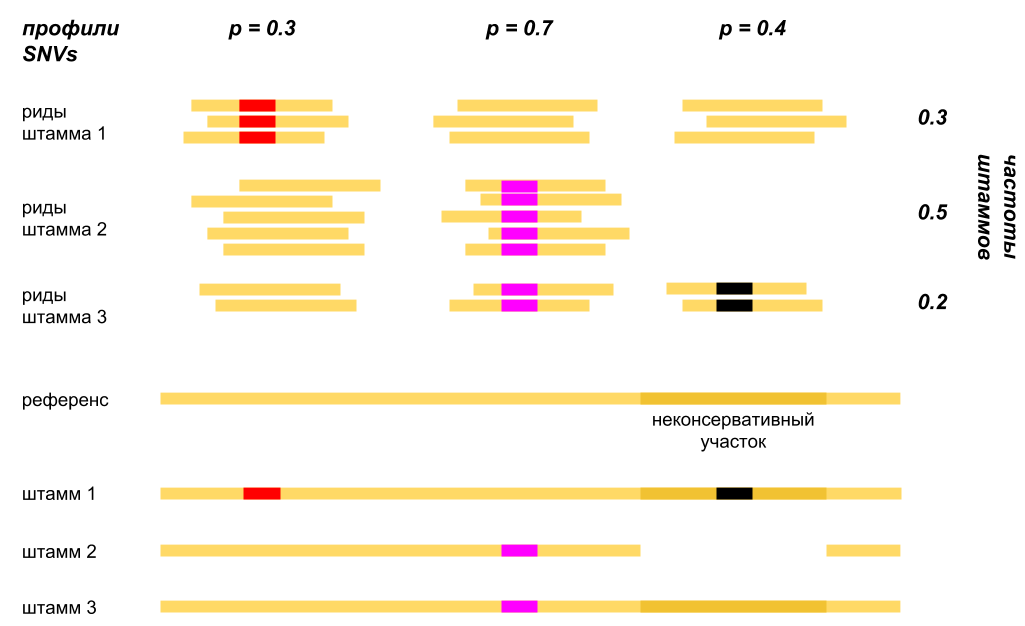
\includegraphics[width=0.9\textwidth]{pics/snv_profiles.png}
\caption{Подсчёт частот однонуклеотидныx мутаций (SNVs) для одного образца. Красным, фиолетовым и чёрным изображены мутации. В середине рисунка схематично представлен участок референсного генома, в нижней части --- соответствующие ему участки геномов штаммов, присутствующих в образце. Первая мутация присутствует только в штамме 1, поэтому её частота соотносится с частотой этого штамма. Вторая мутация присутствует в штаммах 2 и 3, поэтому её частота соотносится с суммоой частот штаммов 2 и 3. Третья мутация попадает на участок, отсутствующий в штамме 2, поэтому её частота не соотносится с суммой частот каких-либо штаммов.}
\label{snv_profile}
\end{figure}

 
Перед тем, как использовать DESMAN для анализа штаммов определенного микроорганизма, пользователь должен тем или иным способом выявить набор соответствующих ему последовательностей (контигов или генов).
DESMAN детектирует SNV относительно найденных в этих последовательностях однокопийных консервативных генов (которые скорее всего присутствуют в каждом из штаммов в единственном экземпляре, --- для этого этапа используется база NCBI COG database) и выясняет их частоты. 
Затем на основании частот SNV с привлечением Байесовской модели, обученной методом Монте Карло по схеме марковской цепи, DESMAN выводит предполагаемое количество штаммов и профили их частот. На следующем этапе для каждого из генов, не являющегося консервативным (такого, который может отсутствовать в одном или нескольких штаммах) DESMAN предсказывает подмножество включающих его штаммов. Так как данная процедура основывается исключительно на профилях покрытия генов, то её без изменений можно применять для анализа других однокопийных фрагментов. 

Отметим, что на сегодняшний момент DESMAN --- единственный инструмент, который позволяет определять генетический состав индивидуальных штаммов среди смеси штаммов, присутствующих в метагеномной серии (упомянутые выше более ранние работы ConStrains~\cite{Constrains} и Lineage~\cite{Lineage} выясняют только процентное соотношение штаммов). Такая функциональность даёт возможность для анализа структурных и фенотипических различий близкородственных штаммов в образцах.

Но заметим, что в случае, если в гене одного из штаммов произойдёт потеря части последовательности или вставка нового элемента, этот ген окажется в сборке фрагментированным, и тогда DESMAN не сможет его обработать. Чтобы объединить фрагменты гена и включить варианты этого гена в итоговый анализ, можно использовать граф сборки, который кодирует потенциальные связи между фрагментами собираемых геномов.



%\subsection{Методы}
\subsection{Графы сборки}

\textit{Графом де Брюина}, построенном по множеству строк S, будем называть граф, вершины которого соответствуют всем возможным k-мерам (последовательность из k символов), присутствующим в S, а направленное ребро соединяет вершину $a$ с вершиной $b$ в том и только том случае, если последние $k - 1$ символов вершины $a$ равны первым $k - 1$ символам вершины $b$.

\textit{Сжатым графом де Брюина} будем называть граф, получаемый из графа де Брюина путём итеративного объединения всех пар вершин $(u, v)$ таких, что из $u$ выходит единственное ребро, идущее в $v$, которое также является единственным входящим ребром для $v$. Вершины $u$ и $v$ удаляются из графа, и добавляется новая вершина $w$, набор входящих рёбер которой равен набору входящих рёбер $u$, набор исходящих -- набору исходящих рёбер $v$. Последовательность символов, соответствующая $w$, получается путём присоединения к последовательности $u$ всех символов $v$, кроме первых~k~-~1.

Значительно упрощая, можно считать, что \textit{граф сборки}, с которым нам в дальнейшем предстоит работать, строится 
следующим образом:
\begin{enumerate}
    \item по множеству ридов строится граф де Брюина;
    \item по графу де Брюина строится сжатый граф де Брюина;
    \item так как в ридах содержатся ошибки секвенирования, далее из сжатого графа де Брюина удаляются элементы, с большой вероятностью порождаемые этими ошибками.
\end{enumerate}
Последовательности, соответсвующие вершинам в графе сборки, называются \textit{юнитигами}.

Если все участки генома были покрыты ридами, а в процессе упрощения графа были удалены только вершины, соответствующие ошибкам секвенирования, то в графе существует путь, последовательность юнитигов которого соответствует геному. После построения графа сборки сборщики ищут такие пути или хотя бы их фрагменты, а также используют дополнительную информацию (например, парность ридов), чтобы объединить юнитиги в более длинные последовательности --- \textit{контиги}.

%На сегодняшний момент нам известен только один инструмент, использующий структуру графа сборки для анализа смесей близкородственных штаммов, --- это MaryGold \cite{MaryGold}, но он только ищет набор мест в графе, соответствующих вариациям между штаммами. 

\subsection{Цель работы}
Целью данной работы является разработка метода, который дополнял бы ответ DESMAN о геномном составе каждого из штаммов в рассматриваемой смеси, выделяя на основе структуры графа сборки более продолжительные регионы, соответствующие каждому штамму. 

Результат поиска таких регионов даст возможность анализировать гены, попавшие в геномные регионы, вариабельные между близкородственными штаммами.


%______________________________________________________________________________

\section{Краткое описание подхода}

В данной работе мы будем анализировать графы сборки, полученные с помощью программы metaSPAdes \cite{MetaSpades}. Настройки этапа <<упрощения>> графа были модифицированы с целью сохранения как можно большего числа вершин, представляющих значимые отличия между штаммам (по умолчанию metaSPAdes стремится в первую очередь обеспечить реконструкцию наиболее высоко-представленного штамма). 

Заметим, что при обработке метагеномных серий многие исследования объединяют риды различных образцов и делают их совместную сборку. 
В частности это позволяет обеспечить реконструкцию геномов, малопредставленных отдельно в каждом их образцов.
В данной работе мы также используем стратегию совместной сборки.

После этапа сборки мы фиксируем вид, для которого в дальнейшем будет проводиться анализ, и отбираем соответствующие ему контиги. В данной работе мы будем считать, что интересующий вид нам уже известен (обозначим его $\mathcal{B}$).

Далее из графа метагеномной сборки мы выделяем подграф, соответствующий зафиксированному виду (обозначим его $G_0$). На алгоритме решения данной задачи мы не будем останавливаться подробно, но предложим некоторые пути решения.

После выделения подграфа и контигов интересующего вида мы проводим поиск SNVs и их частот. Далее мы используем DESMAN для того, чтобы найти количество штаммов и их процентное соотношение. 

Затем мы используем модуль gene-assign программы DESMAN, чтобы определить, каким штаммам принадлежат вершины графа сборки, соответствующие длинным юнитигам. Введение порогового значения на минимальную длину рассматриваемых юнитигов (в текущих экспериментах 1кб) позволяет: 
\begin{enumerate}
    \item исключить из рассмотрения большинство геномных повторов, для которых не предназначен модуль gene-assign  (работа \cite{repeats} показывает, что среди рассмотренных авторами 613 эукариотических видов длина 95\% найденных ими видоспецифичных повторов не превосходит 1кб);
    \item обеспечить более точное соответствие средней глубины покрытия рассматриваемых вершин среднему значению по геному.
\end{enumerate}
 
Наши эксперименты показали, что на тестовых данных классификация DESMAN даёт достаточно мало ложноположительных (False Positive) и ложноотрицательных (False Negative) результатов. Таким образом далее нашей основной задачей является получение ответа для более коротких юнитигов, и это мы делаем, основываясь на структуре графа.

В следующих секциях рассмотрим описанные этапы подробнее.


\section{Первоначальная классификация вершин с помощью DESMAN}

\subsection{Поиск SNVs и их частот}

Пусть мы уже выделили подграф $G_0$, соответствующий $\mathcal{B}$.

Осуществим поиск SNVs. На данном этапе можно использовать референсный геном в случае, если он известен. Иначе можно использовать длинные юнитиги $G_0$.

Для выравнивания ридов мы использовали программу BWA-MEM \cite{bwa_mem}. Для поиска SNVs --- инструмент VarScan \cite{VarScan}, включающий несколько статистических тестов для <<фильтрации>> позиций, наблюдаемые отличия в которых не являются достоверными свидетельствами наличия мутации (могут быть объяснены присутствием ошибок секвенирования). 

Отдельно отметим, что на этом этапе можно оценить, присутствует ли в принципе в образцах смесь близкородственных штаммов интересующего вида (см. Приложение~\ref{dominated_samples}).

\subsection{Дополнительная фильтрация SNVs} 

Будем называть \textit{покрытием позиции} генома число её прочтений ридами при секвенировании. \textit{Покрытием фрагмента} будем называть среднее покрытие по всем его позициям. Оценить покрытие можно, прикладывая риды к референсной последовательности.

Чтобы правильно вывести из частот SNVs частоты штаммов, необходимо брать только те позиции в геноме, которые не попадают на плохо покрытые участки, не принадлежат повторам и при этом присутствуют во всех штаммах рассматриваемого вида (см. пример на Рис. \ref{snv_profile}). Поэтому мы проводим дополнительную фильтрацию SNVs, найденных с помощью VarScan. Кроме того данная процедура позволяет уменьшить размер входа для DESMAN, что существенно ускоряет его работу.

Мы предполагаем, что медиана покрытий всех найденных позиций с SNVs в каждом образце отражает реальное суммарное среднее покрытие однокопийных консервативных регионов рассматриваемых штаммов. 

Мы считаем евклидово расстояние между медианой и покрытием каждой позиции SNVs, после чего оставляем 3000 SNVs, покрытие которых к медиане ближе всех (но это число можно менять в зависимости от условий, таких как степень родства штаммов и количество образцов).

\subsection{Количество штаммов и профили их частот}

Для отобранных SNVs мы считаем вектора частот, после чего применяем DESMAN для того, чтобы определить количество близкородственных штаммов и их процентное соотношение для всех образцов. 

Несмотря на то, что количество штаммов является входным параметром модели, используемой DESMAN, авторами был предложен способ определения <<оптималього>> числа штаммов как значения, начиная с которого график среднего апостериорного отклонения, построенный по результатам запусков программы с разным параметром числа штаммов, перестаёт значительно убывать. 

Мы используем результаты данного этапа DESMAN, предполагая, что они весьма точные. Далее мы приведём результаты экспериментов, подтверждающие это.

\subsection{Классификация вершин графа сборки}

Чтобы получить профиль покрытия каждого юнитига, мы использовали внутренние инструменты пакета SPAdes для вычисления среднего k-мерного покрытия юнитига в каждом из образцов. Оценка среднего нуклеотидного покрытия соответствующего региона может быть затем получена по формуле $\frac{C_k r}{r - k + 1}$, где $C_k$ --- k-мерное покрытие, а $r$ -- средняя длина ридов. 

Используя покрытия длинных юнитигов (больше 1кб), мы запускаем для них процедуру DESMAN gene-assign.
Наши эксперименты на тестовых данных показали, что доля правильных ответов для длинных юнитигов на данном этапе DESMAN также очень высока.
% * <novmargo@gmail.com> 05:41:06 13 Jun 2018 UTC+0300:
% ???




\section{Уточнение классификации с использованием структуры графа}

Методы, описанные в данном разделе, основаны на нескольких предположениях: 
\begin{enumerate}
    \item Граф сборки не содержит <<разрывов>>: каждый штамм соответствует непрерывному пути в графе.
    \item Первичная классификация длинных вершин с помощью процедуры DESMAN gene-assign не содержит ложноположительных резултатов: все длинные юнитиги, классифицированные процедурой DESMAN gene-assign как принадлежащие определенному штамму S, действительно лежат на соответствующем ему пути в графе. 
\end{enumerate}

Нашей целью на этом этапе является идентификация вершин, которые также лежат на пути, соответствующем S. Несмотря на то, что на практике оба предположения не выполняются полностью, далее мы покажем что предсказанные на их основе вершины с высокой вероятностью тоже принадлежат штамму S.

\subsection{Однозначное продолжение пути в графе}

Рассмотрим варианты продолжения пути из вершины $v$, согласно первичной классификации принадлежащей штамму S.

Если $v$ имеет исходящую степень 1, то путь штамма продолжается дальше через единственного её соседа, и его мы можем классифицировать его тоже как принадлежащего штамму S.
В противном случае будем говорить, что $v$ представляет \textit{развилку}.


\begin{figure}[b]
\centering
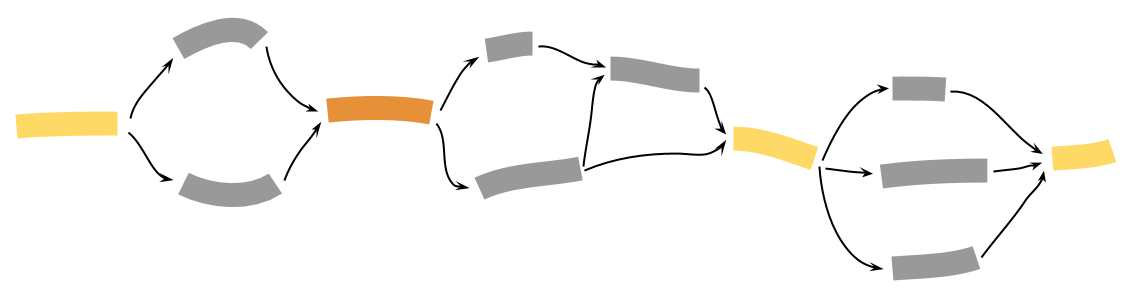
\includegraphics[width=0.8\textwidth]{pics/bubbles_chain.png}
\caption{Цепочка пузырей. Если оранжевая вершина принадлежит штамму, то жёлтые тоже должны ему принадлежать.}
\label{bubbles_chain}
\end{figure}


\begin{figure}[t]
\centering
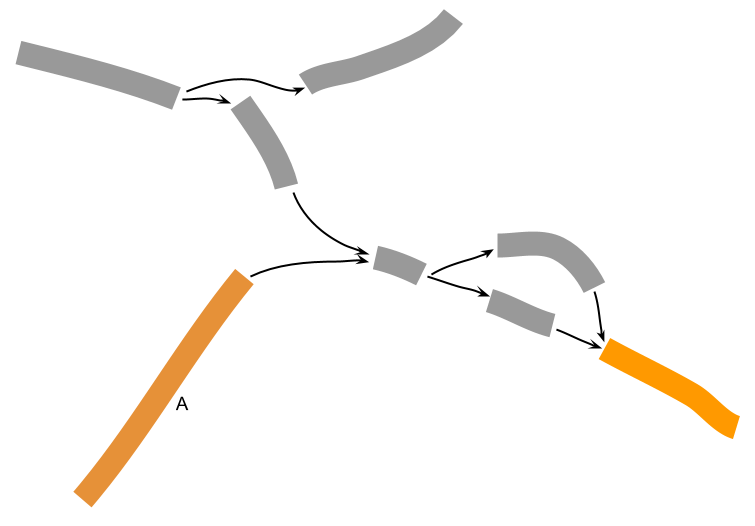
\includegraphics[width=0.57\textwidth]{pics/one_continue.png}
\caption{У вершины $A$ только одно продолжение}
\label{one_continue}
\end{figure}


\subsection{<<Перепрыгивание>> через пузыри}

Было отмечено, что значительная часть развилок в графе соответствует геномным регионам, представляющим отличия между штаммами.

Большая часть таких отличий приводит к появлению в графе так называемых <<суперпузырей>> -- направленных ациклических подграфов с выделенными вершинами <<начала>> и <<конца>>). Говоря неформально, пути, выходящие из начала суперпузыря, могут идти по разным вершинам, но потом вновь сходятся в его конце.  

Поиску и анализу подобных подграфов посвящено несколько работ, например \cite{superbubbles, MaryGold, cacti}.

Следуя работе \cite{superbubbles}, мы определяем понятие \textit{суперпузыря} таким образом. Если упорядоченная пара вершин $(s,t)$ удовлетворяет следующим свойствам:
\begin{enumerate}
    \item $t$ достижима из $s$;
    \item набор вершин, достижимых из $s$ без прохождения через вершину $t$ совпадает с набором вершин, из которых достижима $t$ без прохождения через вершину $s$;
    \item подграф, индуцированный набором $U$ вершин из предыдущего условия является ациклическим;
    \item ни одна вершина из $U$, кроме $t$, не образует с $s$ пары, удовлетворяющей предыдущим условиям;  
\end{enumerate}
то множество $U \cup \{s,t\}$ образуют \textit{суперпузырь}, а $s$ и $t$ --- это его начало и конец соответственно. Далее для краткости мы будем называть \textit{суперпузырь} просто \textit{пузырём}.

Авторы \cite{superbubbles} также предложили простой алгоритм, основанный на топологической сортировке, который для каждой вершины $s$ за константное время в среднем определяет, является ли она началом \textit{суперпузыря}, и если это так, то возвращает его конец $t$ и множество U.

Важное наблюдение заключается в том, что если начало пузыря принадлежит штамму S, то его конец тоже должен принадлежать ему. 

Таким образом итоговая стратегия выглядит следующим образом.
Для каждого штамма S мы рассматриваем все вершины $v$, принадлежащие ему согласно текщей. Далее:
\begin{enumerate}
    \item Проверяем, равна ли исходящая степень вершины 1? Если да, помечаем её единственного соседа тоже как принадлежащего штамму S.
    \item Проверяем, является ли вершина $v$ началом пузыря? Если да, помечаем конец пузыря как принадлежащий штамму S, <<перепрыгивая>> таким образом пузырь (см. Рис. \ref{bubbles_chain}).
\end{enumerate}
процедура повторяется до тех пор, пока существует вершина $v$, удовлетворяющее одному из условий.

Заметим, что та же стратегия работает для графа с обратными рёбрами.

\subsection{Глубокий анализ пузырей}

Зная, какое подмножество штаммов проходит через данный пузырь, попытаемся осуществить классификацию внутренних вершин пузыря, используя профили их покрытия.

Каждому штамму в пузыре соответствует некоторый путь между его началом и концом. Заметим, что исходя из свойств пузырей все такие пути в них являются простыми (проходящими по каждой вершине не более одного раза), и нам необходимо найти такие пути, наилучшим образом описывающие наблюдаемые покрытия вершин.

Задача, схожая с поставленной, рассматривалась в серии работ, посвященных реконструкции альтернативных изоформ эукариотических генов на основании серий экспериментов транскриптомного секвенирования (RNA-seq) \cite{flipflop2, other_flows, flipflop1, isolasso}. Если в нашем случае нужно определить, какому набору штаммов принадлежит вершина, то при анализе РНК-изоформ нужно выяснить, какие изоформы принадлежат тому или иному экзону. Далее мы приведём стратегию, родственную работе \cite{isolasso}.

Пусть через пузырь проходит $k$ штаммов, профили которых нам известны. Пусть $P=\{P_1,P_2,...,P_k\}$ --- вектор длины $k$, отражающий пропорции этих штаммов.

Набор $k$ путей, соответствующим штаммам, можно описать бинарной матрицей $\Theta=\{\theta\}$. $\theta_{v}^{s} = 1$, если штамм $s$ проходит через вершину $v$.

Сначала определим суммарное покрытие вариабельного региона, представленного пузырём, во всех штаммах. Вычислим его по формуле взвешенного среднего покрытий начала и конца пузыря: $$cov_{B} = \frac{cov_s l_s + cov_t l_t}{l_s + l_t}$$ где $s$ и $t$ --- начало и конец пузыря, а $l_s$ и $l_t$ --- длины их юнитигов.

Теперь, зная общее покрытие, вычислим теоретическое покрытие в вершине $v$: 
$$cov_{v}^{(0)} = cov_{B} \sum_{s=1}^{k}$$

Наблюдаемое покрытие в вершине $v$ нам известно. Обозначим его $cov_v^{(1)}$.

Тогда введём величину, характеризующую расхождение между теоретическим и наблюдаемым значениями покрытий для данного набора путей:
$$error = \sum_{v \in bubble} ||cov_{v}^{(0)} - cov_{v}^{(1)}||_2^2 \ln l_{v}$$
Множитель $\ln l_v$ введён для того, с большим весом учитывать расхождения для более длинных вершин, наблюдаемые покрытия которых более достоверно отображают теоретическое.

Переберём все варианты путей и их соответствий штаммам и посчитаем для каждого варианта $error$. 
Вариант, дающий минимальное расхождение, будем считать ответом.
К сожалению, количество возможных путей растёт экспоненциально с увеличением числа вершин в пузыре, поэтому таким образом мы не сможем обрабатывать пузыри, содержащие большое количество вершин. 
Но заметим, что процедуры обработки всех пузырей независимы, поэтому алгоритм можно в несколько раз ускорить, сделав его параллельную реализацию.



\section{Результаты}

Мы определяем для каждой вершины графа, какому подмножеству штаммов она принадлежит. Чтобы оценивать качество алгоритма, переформулируем данную цель следующим образом: для каждого штамма S решим задачу \textit{бинарной классификации} --- вершины графа классифицируем на те которые принадлежат и которые не принадлежат S. Принадлежащие S вершины будем называть \textit{положительными}, не принадлежащие --- \textit{отрицательными}.

Введём обозначения. \textit{TP} --- количество правильно классифицированных положительных вершин. \textit{FP} --- количество неверно классифицированных положительных вершин. \textit{FN} --- количество неверно классифицированных отрицательных вершин.

Тогда для классификации штамма S будем вычислять следующие оценки качества:
\begin{enumerate}
    \item \textit{Точность} (precision) --- доля вершин, названных классификатором положительными и при этом действительно являющихся положительными $$\frac{TP}{TP+FP}$$
    \item \textit{Полнота} (recall) --- доля предсказанных положительных вершин от общего количества положительных вершин $$\frac{TP}{TP+FN}$$
    \item Степень покрытия генома (genome fracion) --- доля суммарной длины вершин TP от длины генома S $$\frac{length(TP)}{length(S)}$$
    \item Длина ложноположительных вершин (FP length) --- суммарная длина всех ложноположительных фрагментов
\end{enumerate}

\subsection{Синтетические датасеты}
При разработке и валидации алгоритма активно использовались синтетические наборы данных. 

Стандартным методом получения таких данных является симуляция ридов из набора референсных геномов \cite{DESMAN, CONCOCT}.
Но в данной работе для того чтобы (до какой-то степени) учесть эффекты ошибок секвенирования и неоднородности покрытия, характерных для секвенирования Illumina, было решено применить метод смешивания в разных пропорциях данных секвенирования различных изолятов \textit{Escherichia coli}. 

Были использованы данные из работы \cite{isolates} (NCBI BioProject PRJNA239027), посвященной анализу 6 образцов \textit{E.coli}, изолированных для 6 пациентов с разной степенью заражения крови. 
Важной особенностью этой работы является то, что авторы также осуществили секвенирование изолятов с использованием технологии PacBio. 
Полученные на основании этих данных высококачественные сборки были использованы нами в качестве референсных геномов.

Мы сгенерировали профили частот следующим образом: частота первого штамма $p_1$ выбиралась случайно из равномерного распределения на отрезке $[0;1]$, частота следующего штамма $p_2$ --- из равномерного распределения на отрезке $[0;1-p_1]$ и так далее. Набор штаммов в образце определялся также случайным образом. После генерации всех профилей выполнялась проверка: имеет ли каждый штамм частоту больше 0.5 хотя бы в одном образце, --- если нет, процедура повторялась заново. Мы рассматривали серии из 10 образцов с вариантами количества штаммов от 3 до 5, по два эксперимента на каждое число (в обозначении "gX\_rY" X cоответсвует количеству штаммов, Y --- номеру эксперимента). Получившиеся профили можно посмотреть в Приложении \ref{app:profiles}.

В данных экспериментах мы детектировали SNVs исходя из выравнивания на длинные юнитиги графов сборки.

Во всех наших экспериментах на тестовых данных DESMAN правильно определил количество штаммов. На \ref{fig:sim_dev}) видно, что все графики перестают существенно убывать там, где это ожидается.

Чтобы найти соответствие между штаммами, использовавшимися при генерации данных, и ответом DESMAN, мы перебирали все возможные перестановки найденных профилей и искали такую, которая давала бы наименьшее евклидово расстояние между ожидаемым (использованном при генерации) и полученным перестановкой предсказанным профилями штаммов. Абсолютное отклонение предсказанных профилей штаммов от ожидаемых, усреднённое по всем штаммам и образцам, составило не более 2.5\%, что позволяет нам доверять этому этапу DESMAN.

Для того, чтобы получить достоверную информацию о принадлежности вершины графа тому или иному набору штаммов, референсные последовательности картировались на граф сборки с использованием внутренних инструментов пакета SPAdes. 

В таблице \ref{res_table} приведены усредненные по штаммам оценки качества, введённые выше. Видно, что точность после каждого шага остаётся очень высокой, в то время как полнота и степень покрытия генома растут, так как мы прибавляем к ответу ранее не классифицированные вершины. При этом суммарная длина ложноположительных фрагментов во всех экспериментах, кроме g5\_r1, не превосходит 100кб.

\begin{table}[b!]
\centering
\begin{tabular}{@{}lllllll@{}}
\toprule
эксперимент &  & \begin{tabular}[c]{@{}l@{}}первоначальная\\ классификация\\ DESMAN\end{tabular} & \begin{tabular}[c]{@{}l@{}}дополнение \\ однозначных \\ продолжений\end{tabular} & \begin{tabular}[c]{@{}l@{}}анализ \\ пузырей\end{tabular} \\ \hline
g3\_r1 & precision & 0.99 & 0.99 & 0.99 \\
 & recall & 0.53 & 0.70 & 0.85 \\
 & genome fraction & 0.94 & 0.97 & 0.99 \\
 & FP length (bp) & 15737 & 15737 & 20500 \\\hline
g3\_r2 &  & 0.98 & 0.97 & 0.97 \\
 &  & 0.51 & 0.69 & 0.80 \\
 &  & 0.92 & 0.96 & 0.98 \\
 &  & 82525 & 86837 & 96189 \\\hline
g4\_r1 &  & 0.99 & 0.98 & 0.99 \\
 &  & 0.40 & 0.57 & 0.76 \\
 &  & 0.87 & 0.93 & 0.97 \\
 &  & 31954 & 43172 & 47514 \\\hline
g4\_r2 &  & 0.99 & 0.98 & 0.98 \\
 &  & 0.37 & 0.55 & 0.79 \\
 &  & 0.91 & 0.93 & 0.97 \\
 &  & 49077 & 66883 & 81964 \\\hline
g5\_r1 &  & 0.97 & 0.96 & 0.97 \\
 &  & 0.26 & 0.41 & 0.67 \\
 &  & 0.80 & 0.88 & 0.93 \\
 &  & 94219 & 126654 & 139414 \\\hline
g5\_r2 &  & 0.99 & 0.99 & 0.99 \\
 &  & 0.26 & 0.42 & 0.67 \\
 &  & 0.77 & 0.88 & 0.93 \\
 &  & 33686 & 38842 & 48475
\end{tabular}
\caption{Результаты экспериментов для синтетических данных. Обозначения: \textit{precision} --- точность, \textit{recall} --- полнота, \textit{genome fraction} --- доля правильно классифицированных нуклеотидов по отношению к длине референса, \textit{FP length} --- суммарная длина ложноположительных фрагментов. Каждая величина усреднена по всем штаммам в эксперименте.}
\label{res_table}
\end{table}

\begin{figure}
    \centering
    
   \begin{subfigure}[b]{0.4\textwidth}
        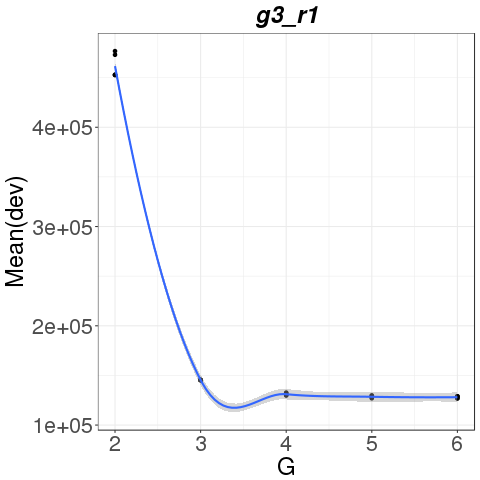
\includegraphics[width=\textwidth]{pics/devs/g3_r1.png}
    \end{subfigure}
    \qquad
    \begin{subfigure}[b]{0.4\textwidth}
        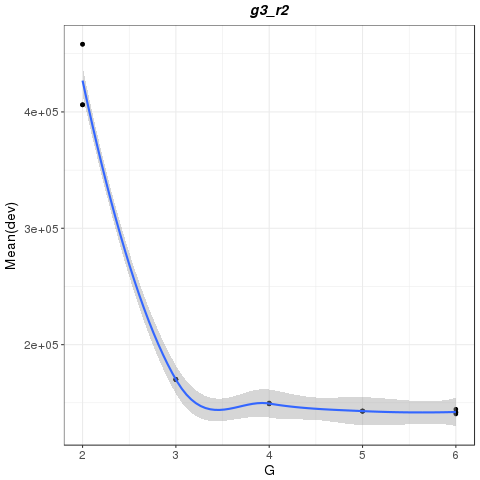
\includegraphics[width=\textwidth]{pics/devs/g3_r2.png}
    \end{subfigure}
      
    \hfill
      
   \begin{subfigure}[b]{0.4\textwidth}
        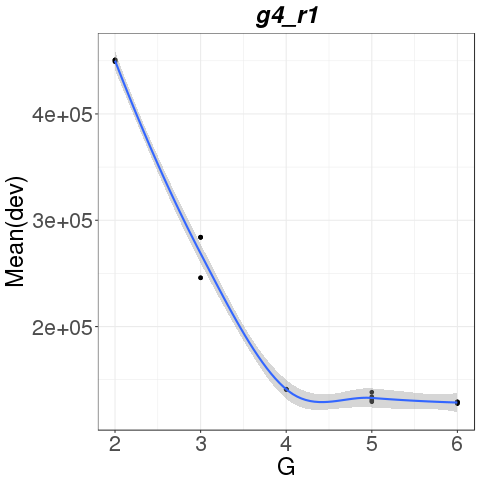
\includegraphics[width=\textwidth]{pics/devs/g4_r1.png}
    \end{subfigure}
    \qquad
    \begin{subfigure}[b]{0.4\textwidth}
        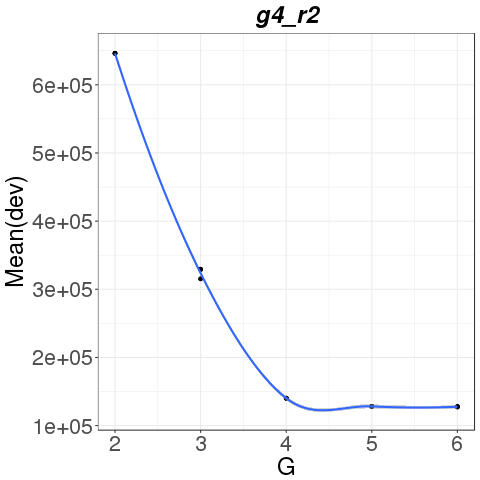
\includegraphics[width=\textwidth]{pics/devs/g4_r2.png}
    \end{subfigure}
      
    \hfill
      
   \begin{subfigure}[b]{0.4\textwidth}
        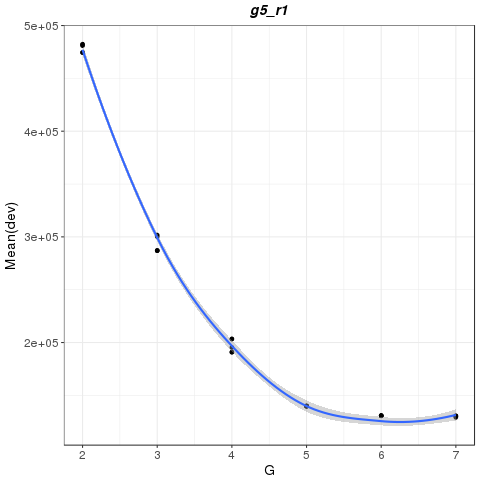
\includegraphics[width=\textwidth]{pics/devs/g5_r1.png}
    \end{subfigure}
    \qquad
    \begin{subfigure}[b]{0.4\textwidth}
        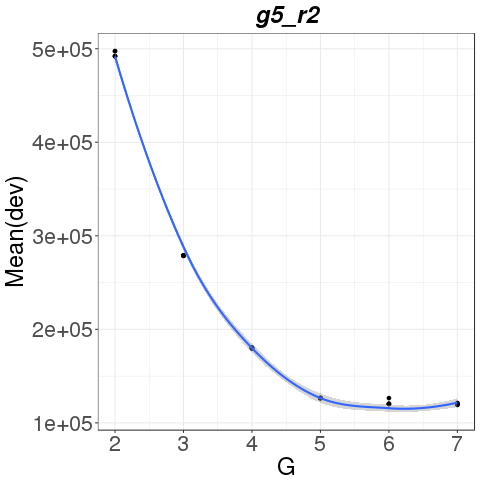
\includegraphics[width=\textwidth]{pics/devs/g5_r2.png}
    \end{subfigure}
    
    \caption{Среднее апостериорное отклонение в зависимости от количества штаммов в синтетических данных.}
    \label{fig:sim_dev}
\end{figure}



%\subsection{Датасет Strain Mock}


\subsection{Набор данных микробиоты младенца} \label{infant_gut_section}

В работе \cite{infant_gut} авторы собрали и просеквенировали 11 фекальных образцов, собранных у недоношенного ребёнка в течение первого месяца жизни. С помощью тщательного и трудоёмкого исследования авторам удалось найти в образцах три штамма \textit{Staphylococcus epidermidis}, оценить их процентное соотношение в каждом из образцов и осуществить качественную реконструкцию двух из них (обозначим эти сборки, согласно оригинальной статье, s1 и s3).

Мы детектировали SNVs исходя из выравнивания ридов на референс \textit{S.epidermidis} из базы данных MIDAS \cite{midas}. Анализ количества штаммов с помощью DESMAN показал, что в данных присутствуют 4 штамма \textit{S.epidermidis} (см. Рис. \ref{infant_gut_figs}). Этот же результат подтверждала наша предыдущая работа, основанная на анализе кластеров частот SNVs, которую мы проводили до интеграции DESMAN в наш подход.

Тем не менее сравнение профилей частот из оригинального исследования и профилей, полученных DESMAN (см. Рис. \ref{infant_gut_figs}), позволяет выявить соответствие между двумя штаммами, найденными DESMAN, и штаммами, для которых доступны сборки s1 и s3. Поэтому мы предполагаем, что можем использовать эти сборки в качестве референсных значений для проверки алгоритма на двух их четырёх штаммов.

Опишем, как мы выделили из графа сборки подграф, соответствующий \textit{S.epidermidis}. Вначале провели биннинг длинных вершин (больше 1кб) с помощью CONCOCT. Далее выравняли сборки из статьи на граф и удалили те длинные вершины, которые оказались не покрыты \textit{S.epidermidis} и попали в бины, в которых \textit{S.epidermidis} принадлежало меньше 30\% вершин. После этого мы оставили только компоненту слабой связности, которой принадлежали все вершины \textit{S.epidermidis}. В получившемся графе мы удалили все тупики  короче 500 баз (вершины с нулевой входящей или исходящей степенью) и сжали все возможные вершины. Выравнивание длинных вершин на базу NCBI показало, что в результате мы всё-таки включили в рассмотрение вершины, принадлежищие плазмидам и фагам \textit{S.epidermidis}, а также небольшое количество вершин родственных видов. Заметим, что проведение качественного биннинга является очень сложной задачей, часто требующей дополнительного ручного валидирования, поэтому наш подход безусловно подразумевает дальнейшие серьёзные исследования этого вопроса.

Далее мы запустили наш алгоритм на получившемся подграфе и рассмотрели результаты для штаммов, соответствующих сборкам s1 и s3. Ожидаемо точность сильно упала по сравнению с синтетическими датасетами, что скорее всего обусловлено тем, что в граф попали вершины не только \textit{S.epidermidis}. Доля правильно классифицированных нуклеотидов оказалась, напротив, сильно выше, чем в синтетических данных, что объясняется скорее всего тем, что рассматриваемые штаммы \textit{S.epidermidis} имеют большую степень родства, чем штаммы \textit{E.coli}, поэтому длина вариабельных регионов у них ниже. Тем не менее полнота подход всё ещё позволяет классифицировать большое количество вершин, не классифицированных DESMAN.

\begin{table}[b!]
\centering
\begin{tabular}{lllll}
\hline
штамм &  & \begin{tabular}[c]{@{}l@{}}первоначальная\\ классификация\\ DESMAN\end{tabular} & \begin{tabular}[c]{@{}l@{}}дополнение \\ однозначных \\ продолжений\end{tabular} & \begin{tabular}[c]{@{}l@{}}анализ \\ пузырей\end{tabular} \\ \hline
s1 & precision & 0.76 & 0.76 & 0.76 \\
 & recall & 0.22 & 0.43 & 0.51 \\
 & genome fraction & 0.97 & 0.98 & 0.98 \\
 & FP length (bp) & 166116 & 179318 & 185637 \\\hline
s3 &  & 0.82 & 0.85 & 0.86 \\
 &  & 0.21 & 0.40 & 0.48 \\
 &  & 0.97 & 0.98 & 0.98 \\
 &  & 124450 & 127672 & 128220
\end{tabular}
\caption{Результаты экспериментов для микробиоты младенца. Обозначения: \textit{precision} --- точность, \textit{recall} --- полнота, \textit{genome fraction} --- доля правильно классифицированных нуклеотидов по отношению к длине референса, \textit{FP length} --- суммарная длина ложноположительных фрагментов.}
\label{res_table_ig}
\end{table}

\begin{figure}
    \centering
    \begin{subfigure}[b]{0.7\textwidth}
        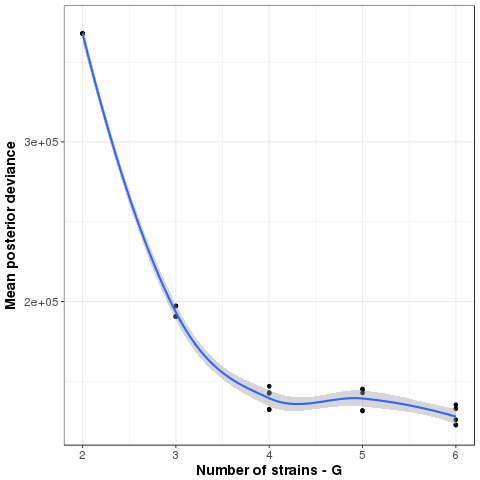
\includegraphics[width=\textwidth]{pics/infant_gut_dev.png}
        \caption{Среднее апостериорное отклонение}
    \end{subfigure}
      
    \hfill
      
    \begin{subfigure}[b]{1.0\textwidth}
        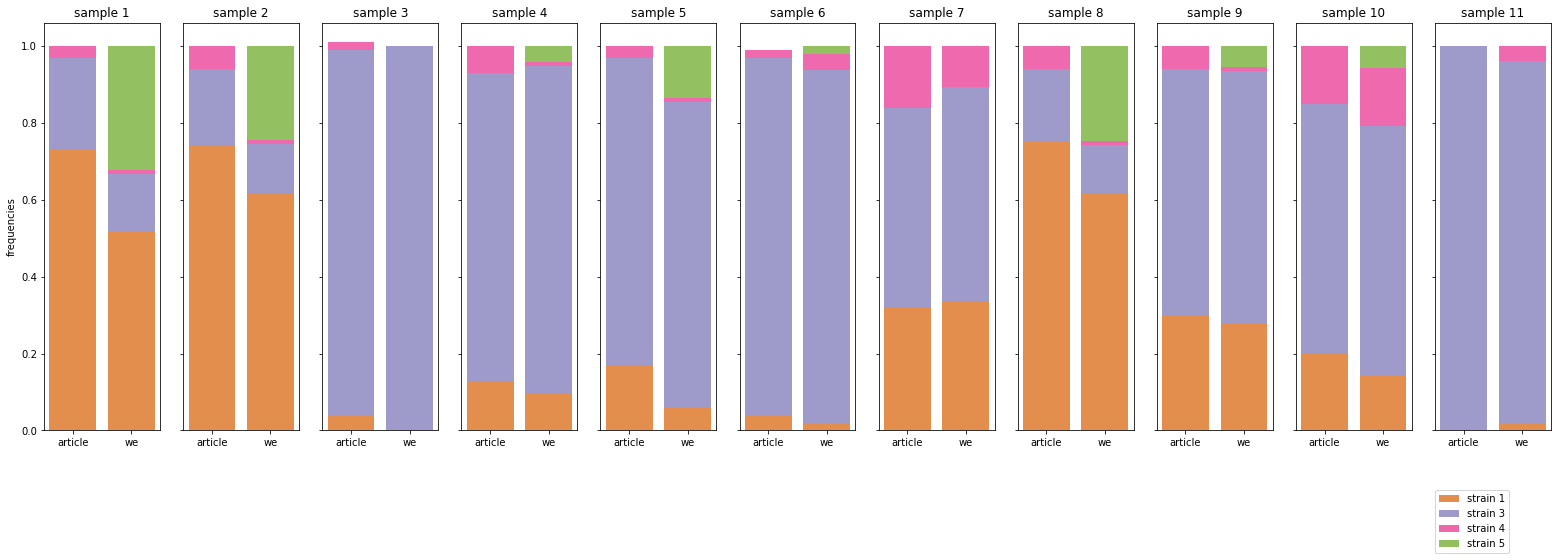
\includegraphics[width=\textwidth]{pics/infant_gut_results.png}
        \caption{Сравнение получившихся частот с оригинальным исследованием}
    \end{subfigure}
    
    \caption{количество и пропорции штаммов \textit{S.epidermidis} в \textit{infant gut}}\label{infant_gut_figs}
\end{figure}


% У заключения нет номера главы
\section*{Заключение}
В данной работе была рассмотрена задача анализа геномного состава каждого из близкородственных штаммов  при наличии смеси таковых в метагеномных сериях. 

Был предложен подход, который классифицирует вершины графа сборки по принадлежности к тому или иному набору штаммов. Алгоритм использует в качестве отправной точки ответ процедуры \textit{gene-assign} инструмента DESMAN для длинных вершин графа и далее распространяет этот ответ на короткие вершины, которые можно классифицировать исходя из структуры графа. Для этого алгоритм ищет вершины, с большой вероятностью лежащие на пути в графе, соответствующем штамму, а также анализирует композицию штаммов в пузырях графа, соответствующих вариабельным участкам.

Было сгенерировано шесть синтетических метагеномных серий, на которых алгоритм показал высокие результаты как по точности, так и по полноте предсказания.

Кроме того было показано, что алгоритм можно применять и к реальным метагеномным данным. 

Разработанный алгоритм позволит улучшить сборку вариабельных регионов геномов близкородственных штаммов и находить больше генов, попадающих на такие участки.

Дальнейшим развитием данной работы может стать улучшение алгоритма для обработки более сложных структур графа, такиx как: пузыри с циклами и тупиками, разрывы из-за низкого покрытия пути, соответствующего геному, циклы, индуцированные повторами.

Кроме того работа только поверхностно затрагивает проблему выделения в метагеномном графе подграфа, соответствующего смеси штаммов, поэтому данный вопрос требует дальнейшего изучения.


\bibliographystyle{ugost2008ls}
\bibliography{diploma.bib}

%\appendix
\begin{appendices}

\section{Проверка образца на наличие смеси близкородственных штаммов}\label{dominated_samples}

Опишем алгоритм поиска образцов с доминантными штаммами некоторого рассматриваемого вида.

В каждом образце найдем однонуклеотидные мутации относительно референса рассматриваемого вида. Для каждой мутации считаем, сколько ридов поддерживает референс, а сколько – мутацию. Чтобы оставить только те мутации, которые не лежат в повторах и малопокрытых участках генома, возьмем только такие, чье суммарное покрытие близко к медиане покрытия этого вида в образце. Для каждой из выбранных мутаций подсчитаем частоту ридов, поддерживающих мутацию.

Каждая мутация специфична для какого-то одного штамма или некоторого множества штаммов. Если мы выбрали мутации с хорошим покрытием и не попадающие в повторы, то частота ридов, поддерживающих эту мутацию, должна примерно соответствовать сумме частот штаммов, для которых специфична эта мутация.

Тогда заметим, что если частота доминантного штамма --- $X$, и $X > 0.7$, то мы должны наблюдать мутации с частотой порядка $X$ и больше. При этом мутации, специфичные только для всех остальных штаммов, не могут давать частоты больше $(1-X)$. Тогда в случае, когда в образце присутствует доминантный штамм, в распределении частот, соответствующих мутациям, мы должны наблюдать отсутствие значений в промежутке $((1-X); X)$.

Найдем величину промежутка эмпирически. Так как границы промежутка должны быть симметричны относительно значения 0.5, начнем с его середины и будем добавлять с обоих концов некоторую маленькую величину $\epsilon$ (например, $0.01$) до тех пор, пока в промежуток попадает не больше $5\%$ от всех значений частот мутаций (те мутации, которые туда попали, считаем погрешностью). После того, как мы нашли предполагаемый промежуток, смотрим на его правую границу. Если она больше $0.7$, считаем, что $X > 0.7$, и в образце есть доминантный штамм. Иначе – доминантного штамма нет.


\section{Профили частот штаммов в синтетических данных}\label{app:profiles}

\begin{table}[!ht]
\centering
\scalebox{0.95}{
\begin{tabular}{llllllllllll}
g3\_r1 &  &  &  &  &  &  &  &  &  &  &  \\
 & s5 & 0.08 & 0.87 & 0.24 & 0.02 & 0.46 & 0.44 & 0.46 & 0.75 & 0.02 & 0.97 \\
 & s4 & 0.73 & 0.12 & 0.37 & 0.26 & 0.47 & 0.56 & 0.01 & 0.14 & 0.01 & 0.03 \\
 & s8 & 0.19 & 0.01 & 0.39 & 0.72 & 0.07 & 0 & 0.53 & 0.11 & 0.97 & 0 \\
 &  &  &  &  &  &  &  &  &  &  &  \\
g3\_r2 &  &  &  &  &  &  &  &  &  &  &  \\
 & s7 & 0.44 & 0.13 & 0.1 & 0.42 & 0.06 & 0.55 & 0.76 & 0.3 & 0.22 & 0.23 \\
 & s9 & 0.55 & 0.84 & 0.11 & 0.53 & 0.12 & 0.32 & 0.14 & 0.2 & 0.78 & 0.1 \\
 & s5 & 0.01 & 0.03 & 0.79 & 0.05 & 0.82 & 0.13 & 0.1 & 0.5 & 0 & 0.67 \\
 &  &  &  &  &  &  &  &  &  &  &  \\
g4\_r1 &  &  &  &  &  &  &  &  &  &  &  \\
 & s7 & 0.19 & 0.23 & 0.43 & 0.93 & 0.82 & 0.57 & 0.89 & 0.64 & 0.04 & 0.05 \\
 & s4 & 0.06 & 0.7 & 0.03 & 0.05 & 0.08 & 0.34 & 0.04 & 0.03 & 0.09 & 0.53 \\
 & s5 & 0.69 & 0.03 & 0.03 & 0.02 & 0.05 & 0.09 & 0.06 & 0.3 & 0.01 & 0.05 \\
 & s8 & 0.06 & 0.04 & 0.51 & 0 & 0.05 & 0 & 0.01 & 0.03 & 0.86 & 0.37 \\
 &  &  &  &  &  &  &  &  &  &  &  \\
g4\_r2 &  &  &  &  &  &  &  &  &  &  &  \\
 & s5 & 0.11 & 0.18 & 0.04 & 0.03 & 0.82 & 0.84 & 0.5 & 0.03 & 0.1 & 0.6 \\
 & s4 & 0.14 & 0.33 & 0.06 & 0.02 & 0.1 & 0.14 & 0.46 & 0.95 & 0.38 & 0.37 \\
 & s9 & 0.12 & 0.15 & 0.12 & 0.92 & 0.02 & 0.02 & 0.01 & 0.01 & 0.49 & 0.01 \\
 & s8 & 0.63 & 0.34 & 0.78 & 0.03 & 0.06 & 0 & 0.03 & 0.01 & 0.03 & 0.02 \\
 &  &  &  &  &  &  &  &  &  &  &  \\
g5\_r1 &  &  &  &  &  &  &  &  &  &  &  \\
 & s5 & 0.97 & 0.61 & 0.34 & 0.01 & 0.35 & 0.57 & 0.14 & 0.19 & 0.2 & 0.89 \\
 & s9 & 0 & 0.16 & 0.08 & 0.06 & 0.24 & 0.22 & 0.16 & 0.75 & 0.07 & 0.08 \\
 & s4 & 0.01 & 0.21 & 0.23 & 0.03 & 0.12 & 0.16 & 0.61 & 0 & 0.01 & 0 \\
 & s7 & 0 & 0 & 0.27 & 0.26 & 0.1 & 0.02 & 0.02 & 0.02 & 0.71 & 0 \\
 & s8 & 0.02 & 0.02 & 0.08 & 0.64 & 0.19 & 0.03 & 0.07 & 0.04 & 0.01 & 0.03 \\
 &  &  &  &  &  &  &  &  &  &  &  \\
g5\_r2 &  &  &  &  &  &  &  &  &  &  &  \\
 & s8 & 0.4 & 0.75 & 0.81 & 0.67 & 0.14 & 0.07 & 0.01 & 0.31 & 0.54 & 0.15 \\
 & s5 & 0.16 & 0 & 0.01 & 0.26 & 0.03 & 0 & 0.28 & 0.54 & 0.28 & 0.76 \\
 & s7 & 0.33 & 0 & 0.14 & 0 & 0.03 & 0.21 & 0.66 & 0 & 0.16 & 0 \\
 & s4 & 0.1 & 0.25 & 0.04 & 0.05 & 0.05 & 0.53 & 0.05 & 0.11 & 0.02 & 0.09 \\
 & s9 & 0.01 & 0 & 0 & 0.02 & 0.75 & 0.19 & 0 & 0.04 & 0 & 0
\end{tabular}
}
\caption{Профили частот штаммов, использовавшихся для генерации синтетических данных.}
\label{table:profiles}
\end{table}

\end{appendices}

\end{document}
